\chapter{Подпространства, операторы проекции и измерение как запутывание}

Теорема Белла оставила открытыми два вопроса. Что остаётся от запутанности, когда один из членов пары возмущён, поглощён или измерен? И что именно превращает обычное взаимодействие в измерение? Путь к ответу лежит через элементарную линейную алгебру. Свойства — это подпространства, вероятности — математические ожидания проекторов, а измерительный прибор — другая квантовая система, с которой объект запутывается.

\section{Вводная мотивация: запутанность, локальность и измерение}

Предположим, синглет разнесён на две удалённые части и одна из них измеряется. Должна ли квантовая теория поля описывать между ними виртуальный обмен? На удалённой стороне не происходит ничего обнаружимого, и никакое пригодное к использованию сообщение туда не приходит. Можно локально повернуть один спин магнитным полем, изменив детальную форму совместного состояния, тогда как степень запутанности при такой локальной операции остаётся неизменной. Количественные меры запутанности появятся позже; сейчас важно, что две системы, которые больше не взаимодействуют, не могут изменить свою общую запутанность лишь посредством операции, ограниченной одной стороной.

\begin{classroomqa}
\lecturetimestamp{00:00:22}
\audiencequestion{Требует ли измерение одного из членов синглета, разделённого пространственноподобным интервалом, некоторого виртуального обмена с другим?}
\lecturerresponse{Нет, на другой стороне не происходит никакого обнаружимого обмена. Локальная операция может повернуть один из факторов и изменить форму, в которой записано совместное состояние, но сама по себе не может ни передать сообщение, ни изменить общую запутанность между разделёнными частями.}
\end{classroomqa}

Это вынуждает расширить представление о том, что считать партнёром. Если один из членов запутанной пары падает в чёрную дыру, второй не перестаёт быть запутанным; он оказывается запутан со степенями свободы чёрной дыры, а после её испарения — с испущенным излучением. Для этой идеи не нужна и чёрная дыра. Бросьте один из членов запутанной пары в ванну и дайте ему бурно перемешаться с водой. Его индивидуальная идентичность может потеряться в многочастичном состоянии, и всё же удалённая частица остаётся запутанной с ванной в целом и в конце концов — с выходящим паром.

Речь идёт не только о сохранении. Речь также идёт об обратимости. Если взаимодействие может создавать запутанность, то оно же в принципе может её и устранять. Распутывание возможно, но только когда системы снова приходят в контакт и вновь взаимодействуют. Всё, что может происходить в одну сторону, может происходить и в другую.

\begin{classroomqa}
\lecturetimestamp{00:04:45}
\audiencequestion{Если измерены оба спина запутанной пары, остаются ли электроны запутанными? Может ли уже одно измерение распутать их?}
\lecturerresponse{Измерения могут устранить их взаимную запутанность, и одного измерения может быть достаточно. Чтобы понять, что означает это утверждение, а не просто постулировать коллапс, нужно описать наблюдение как взаимодействие между системой и регистрирующим прибором.}
\end{classroomqa}

Этот вопрос задаёт цель: связать наблюдение, коллапс волнового пакета и запутанность. Однако прежде чем к ней подойти, нам нужно более ясное изложение подпространств и операторов проекции, не прибегая к более тяжёлому формализму, чем требует рассуждение.

\section{Размерность, линейная зависимость и ортонормированные базисы}

Поэтому пока мы будем оставаться в рамках конечномерных векторных пространств, снабжённых бра, кетами и скалярным произведением. Сасскинд начинает настолько элементарно, насколько это возможно. Он не определяет размерность подсчётом компонент в столбцовом векторе. Он определяет её абстрактно: размерность векторного пространства — это максимальное число линейно независимых векторов, которое можно в нём найти.

Следовательно, набор \(\{|v_i\rangle\}\) линейно независим, если соотношение
\begin{equation}
\sum_i c_i |v_i\rangle = 0
\end{equation}
влечёт обращение в нуль всех коэффициентов \(c_i\). Эквивалентно, ни один из векторов нельзя представить как линейную комбинацию остальных.

Здесь крайне важно, что ортогональность — не то же самое, что независимость. В трёх измерениях можно иметь три вектора, вовсе не ортогональные, и всё же линейно независимые. Важно то, можно ли один из них построить из двух других. С другой стороны, на двумерной плоскости любой третий вектор в этой плоскости обязательно линейно зависит от первых двух.

\begin{figure}[htbp]
\centering
\includegraphics[width=0.56\textwidth]{lecture_06_figure_02.png}
\caption{Три вектора, нарисованные на доске. В лекции этот набросок используется, чтобы отделить идею ортогональности от идеи линейной независимости, а затем подчеркнуть, что на плоскости третий вектор зависит от первых двух.}
\lectureframe{00:09:35}
\end{figure}

\begin{figure}[htbp]
\centering
\begin{tikzpicture}[scale=1.2]
\draw[->] (0,0) -- (2.3,0);
\draw[->] (0,0) -- (2.0,2.0);
\draw[->] (0.35,0.95) -- (1.05,1.45);
\fill (0,0) circle (1.2pt);
\end{tikzpicture}
\caption{Минимальная реконструкция рисунка на доске. Точное соотношение между коэффициентами по одному этому кадру не фиксируется; геометрический смысл состоит в том, что на двумерной плоскости третий вектор не является линейно независимым.}
\end{figure}

В этом и состоит смысл рисунка. Если пространство двумерно, максимальное число линейно независимых векторов равно двум. Если пространство трёхмерно, оно равно трём. В более общем случае, если пространство имеет размерность \(d\), то при заданном скалярном произведении можно найти \(d\) взаимно ортогональных единичных векторов, порождающих его. Это базисные векторы. Сасскинд прямо говорит, что не будет здесь доказывать эту теорему. Ему нужен только вывод: как только такой базис существует, любой вектор пространства можно разложить по нему.

\begin{classroomqa}
\lecturetimestamp{00:10:58}
\audiencequestion{Совпадает ли число пространственных степеней свободы с размерностью пространства состояний?}
\lecturerresponse{Нет. У частицы, движущейся в комнате, есть три пространственные координаты, но огромное число взаимно ортогональных квантовых состояний. Размерность конфигурационного пространства и размерность гильбертова пространства — разные понятия; конечномерные примеры используются лишь для того, чтобы ясно показать логику.}
\end{classroomqa}

\section{Разложение по базису, диады и разложение единицы}

Теперь выберем ортонормированный базис \(\{|n\rangle\}\), где \(n=1,\dots,d\). На этом месте запись на доске особенно ясна и компактна:

\begin{figure}[htbp]
\centering
\includegraphics[width=0.62\textwidth]{lecture_06_figure_03.png}
\caption{Ортонормированный базис и разложение произвольного состояния.}
\lectureframe{00:14:15}
\end{figure}

Пишем
\begin{align}
\langle m|n\rangle &= \delta_{mn}, \\
|\psi\rangle &= \sum_n a_n |n\rangle.
\end{align}
Здесь \(\delta_{mn}\) — это символ Кронекера: он равен \(1\) при \(m=n\) и \(0\) в противном случае.

\paragraph{Подробный вывод.} Коэффициенты восстанавливаются проецированием на базис. Умножим слева на \(\langle m|\):
\begin{align}
\langle m|\psi\rangle
  &= \sum_n a_n \langle m|n\rangle \\
  &= \sum_n a_n \delta_{mn} \\
  &= a_m.
\end{align}
Итак, коэффициенты просто равны
\begin{equation}
a_m = \langle m|\psi\rangle.
\end{equation}
Коэффициент — обычное комплексное число, поэтому его можно поставить по любую сторону кета, ничего не меняя.

Если подставить коэффициент обратно в разложение, получим
\begin{equation}
|\psi\rangle = \sum_n |n\rangle \langle n|\psi\rangle.
\end{equation}
Это подсказывает, что объект \(|n\rangle\langle n|\) и, в более общем виде, \(|a\rangle\langle b|\) следует понимать как оператор. Именно это и делается дальше. Диада действует по правилу
\begin{equation}
\bigl(|a\rangle\langle b|\bigr)|\psi\rangle = \langle b|\psi\rangle\,|a\rangle.
\end{equation}
Бра извлекает комплексное число; кет задаёт результирующее направление. Это простой путь Сасскинда от векторов к операторам.

Теперь прочитаем предыдущее разложение как операторное равенство. Поскольку
\begin{equation}
|\psi\rangle = \left(\sum_n |n\rangle\langle n|\right)|\psi\rangle
\end{equation}
для любого \(|\psi\rangle\), оператор в скобках должен быть тождественным оператором:
\begin{equation}
\sum_n |n\rangle\langle n| = I.
\end{equation}
Это и есть разложение единицы.

\begin{figure}[htbp]
\centering
\includegraphics[width=0.60\textwidth]{lecture_06_figure_07.png}
\caption{Завершённая запись разложения единицы на доске.}
\lectureframe{00:18:30}
\end{figure}

\begin{classroomqa}
\lecturetimestamp{00:18:39}
\audiencequestion{Должны ли векторы в разложении единицы образовывать базис?}
\lecturerresponse{Да. В выводе использовались и нормировка, и взаимная ортогональность, а суммирование должно вестись по полному базису. Произвольный набор векторов не даёт разложения единицы.}
\end{classroomqa}

Тождественный оператор сам является проектором на всё пространство. Каждый вектор является собственным вектором \(I\), и каждое собственное значение равно \(+1\).

\begin{classroomqa}
\lecturetimestamp{00:19:14}
\audiencequestion{Означает ли разложение единицы, что у каждого вектора собственное значение равно единице?}
\lecturerresponse{Да, для тождественного оператора. Он исключителен тем, что каждый вектор является его собственным вектором и \(I|\psi\rangle=|\psi\rangle\) для любого состояния.}
\end{classroomqa}

\section{Свойства как подпространства и операторы проекции}

Имея в распоряжении этот аппарат, лекция вносит своё главное концептуальное уточнение. Свойство вроде \(k=\lambda\) — это, вообще говоря, не один вектор. Это целое подпространство.

Пусть \(k\) — эрмитова наблюдаемая и предположим
\begin{equation}
k|A\rangle = \lambda |A\rangle, \qquad
k|B\rangle = \lambda |B\rangle,
\end{equation}
где \(|A\rangle\) и \(|B\rangle\) линейно независимы. Тогда любая линейная комбинация имеет то же собственное значение:
\begin{align}
k\bigl(\alpha|A\rangle+\beta|B\rangle\bigr)
  &= \alpha k|A\rangle + \beta k|B\rangle \\
  &= \alpha \lambda |A\rangle + \beta \lambda |B\rangle \\
  &= \lambda\bigl(\alpha|A\rangle+\beta|B\rangle\bigr).
\end{align}
Следовательно, собственное подпространство, соответствующее \(\lambda\), замкнуто относительно сложения и умножения на скаляр. Это векторное подпространство.

Первый конкретный пример в лекции — двухспиновая система. Состояния
\begin{equation}
|ud\rangle,\qquad |uu\rangle
\end{equation}
имеют разные значения второго спина, но одно и то же значение первого: в обоих случаях первый спин направлен вверх. Поэтому они порождают подпространство, в котором \(\sigma_3=+1\) для первого спина.

\begin{figure}[htbp]
\centering
\includegraphics[width=0.46\textwidth]{lecture_06_figure_04.png}
\caption{Два двухспиновых состояния с первым спином вверх.}
\lectureframe{00:23:27}
\end{figure}

Вот что стоит сохранить: свойство — это не обязательно одно состояние. Это целая совокупность состояний с одним и тем же собственным значением.

Чтобы избежать путаницы в обозначениях, которая ненадолго возникает на доске, мы сохраним заглавные буквы \(A,B,\dots\) для конкретных собственных векторов, а строчные \(a,b,\dots\) будем использовать как индексы суммирования, пробегающие ортонормированный базис собственного подпространства. Если \(\{|a\rangle\}\) — такой базис для подпространства \(k=\lambda\), то оператор проекции на это подпространство равен
\begin{equation}
\Pi_{k=\lambda}=\sum_a |a\rangle\langle a|.
\end{equation}
Это просто единичный оператор, ограниченный данным подпространством. Если \(|\psi\rangle\) уже лежит в нем, проектор оставляет его без изменения. Если \(|\psi\rangle\) частично лежит вне него, проектор отбрасывает ортогональный остаток и сохраняет только компоненту внутри.

\section{Постулат вероятности, совместимые свойства и повторение теоремы Белла}

После того как свойства переосмыслены как подпространства, постулат вероятности принимает наиболее ясную форму. Если \(|\psi\rangle\) нормирован, то вероятность того, что он обладает свойством \(k=\lambda\), равна
\begin{equation}
P(k=\lambda)=\langle\psi|\Pi_{k=\lambda}|\psi\rangle.
\end{equation}

\begin{figure}[htbp]
\centering
\includegraphics[width=0.58\textwidth]{lecture_06_figure_05.png}
\caption{Проектор на собственное подпространство \(k=\lambda\). Расположение на доске уже подготавливает следующий шаг: поместить проектор между \(\langle\psi|\) и \(|\psi\rangle\).}
\lectureframe{00:31:09}
\end{figure}

Подставим диадическую форму проектора:
\begin{align}
P(k=\lambda)
  &= \left\langle \psi \left| \sum_a |a\rangle\langle a| \right| \psi \right\rangle \\
  &= \sum_a \langle\psi|a\rangle\langle a|\psi\rangle \\
  &= \sum_a |\langle a|\psi\rangle|^2.
\end{align}
Это в точности та интерпретация, которая дается в лекции: полная вероятность данного свойства есть сумма вероятностей всех ортогональных способов, которыми это свойство может реализоваться.

В двухспиновой системе для случая, когда первый спин направлен вверх, соответствующее подпространство натянуто на \(|uu\rangle\) и \(|ud\rangle\), так что
\begin{equation}
\Pi_{\sigma_3=+1}=|uu\rangle\langle uu|+|ud\rangle\langle ud|.
\end{equation}
В сокращенной записи лекции это также пишется как
\begin{equation}
\Pi_{\sigma_3=+1}=\frac{1+\sigma_3}{2},
\end{equation}
где единичный оператор на втором спине опущен.

\begin{classroomqa}
\lecturetimestamp{00:33:04}
\audiencequestion{В чем разница между наблюдаемой, свойством и проектором?}
\lecturerresponse{Наблюдаемая — это эрмитов оператор \(k\). Свойство \(k=\lambda\) представляется собственным подпространством и означает, что измерение \(k\) наверняка дало бы \(\lambda\). Проектор \(\Pi_{k=\lambda}\) выделяет это подпространство, а его среднее значение дает вероятность наличия этого свойства.}
\end{classroomqa}

\begin{classroomqa}
\lecturetimestamp{00:34:07}
\audiencequestion{Обязательно ли вырожденные собственные векторы \(A\) и \(B\) уже должны быть ортогональны, и образуют ли они базис всего пространства?}
\lecturerresponse{Исходные собственные векторы не обязаны быть ортогональными, но внутри их собственного подпространства всегда можно выбрать ортонормированный базис. Это базис только для данного подпространства; чтобы натянуть все пространство, нужны дополнительные ортогональные направления. Проецирование на каждый базисный вектор подпространства с последующим суммированием дает проекцию на это подпространство.}
\end{classroomqa}

\begin{classroomqa}
\lecturetimestamp{00:35:33}
\audiencequestion{Означает ли символ \(a\) в \(k|A\rangle=\lambda|A\rangle\) то же самое, что и \(a\), по которому ведется суммирование в проекторе?}
\lecturerresponse{Нет. Первое обозначение относится к конкретному собственному вектору, тогда как индекс под знаком суммы пробегает все векторы ортонормированного базиса собственного подпространства. Различные обозначения не позволяют спутать фиксированную метку с фиктивным индексом суммирования.}
\end{classroomqa}

\begin{classroomqa}
\lecturetimestamp{00:37:15}
\audiencequestion{Являются ли скалярные произведения в формуле проектора вероятностями или амплитудами вероятности?}
\lecturerresponse{Каждое \(\langle a|\psi\rangle\) — это амплитуда. Умножение на комплексно-сопряженную величину дает вероятность, а суммирование этих вероятностей по ортогональным способам реализации \(k=\lambda\) дает полную вероятность свойства.}
\end{classroomqa}

Затем в лекции ставится вопрос, как комбинировать свойства. Предположим, у нас есть два совместимых свойства, представленных коммутирующими проекторами \(P_k\) и \(P_\ell\). На языке лекции высказывание И представляется произведением:
\begin{equation}
\Pi_{k=\lambda\,\wedge\,\ell=\mu}=P_kP_\ell=P_\ell P_k.
\end{equation}
Логика проста. \(P_k|\psi\rangle\) лежит в подпространстве \(k=\lambda\). Поскольку операторы коммутируют, \(P_\ell P_k|\psi\rangle=P_kP_\ell|\psi\rangle\), так что тот же вектор лежит и в подпространстве \(\ell=\mu\). Следовательно, произведение проецирует на совместное свойство. Соответствующая вероятность равна
\begin{equation}
P(k=\lambda,\ell=\mu)=\langle\psi|P_kP_\ell|\psi\rangle.
\end{equation}

Первый шаг в этом рассуждении стоит выписать отдельно. Для любого состояния
\begin{equation}
k\bigl(P_k|\psi\rangle\bigr)=\lambda P_k|\psi\rangle,
\end{equation}
следовательно, \(P_k|\psi\rangle\) лежит в собственном подпространстве \(k=\lambda\). Если \(P_k\) и \(P_\ell\) коммутируют, результат их действия можно записать, поставив слева любой из проекторов, и потому получающийся вектор принадлежит обоим подпространствам.

\begin{figure}[htbp]
\centering
\includegraphics[width=0.44\textwidth]{lecture_06_figure_06.png}
\caption{Спроецированное состояние как вектор в собственном подпространстве.}
\lectureframe{00:41:57}
\end{figure}

\begin{figure}[htbp]
\centering
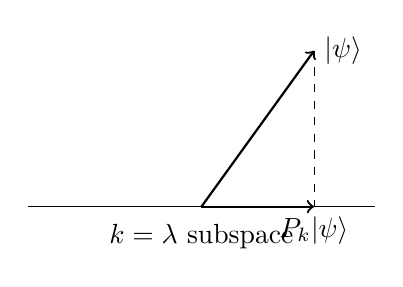
\begin{tikzpicture}[scale=1.1]
\draw (-2,0) -- (2,0);
\draw[->,thick] (0,0) -- (1.3,1.8) node[right] {$|\psi\rangle$};
\draw[dashed] (1.3,1.8) -- (1.3,0);
\draw[->,thick] (0,0) -- (1.3,0) node[below] {$P_k|\psi\rangle$};
\node at (0,-0.35) {$k=\lambda$ subspace};
\end{tikzpicture}
\caption{Проецирование произвольного вектора в собственное подпространство \(k=\lambda\).}
\end{figure}

\begin{figure}[htbp]
\centering
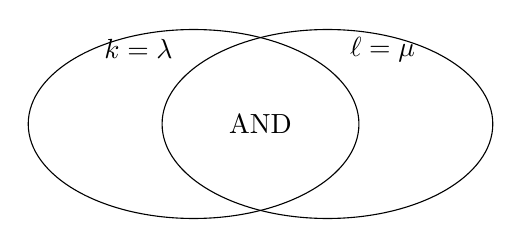
\begin{tikzpicture}[scale=1.0]
\draw (0,0) ellipse (2.1 and 1.2);
\draw (1.7,0) ellipse (2.1 and 1.2);
\node at (-0.7,0.95) {$k=\lambda$};
\node at (2.4,0.95) {$\ell=\mu$};
\node at (0.85,0) {AND};
\end{tikzpicture}
\caption{Реконструкция картины пересекающихся подпространств, лежащей в основе высказывания И для коммутирующих проекторов.}
\end{figure}

\begin{figure}[htbp]
\centering
\includegraphics[width=0.66\textwidth]{lecture_06_figure_08.png}
\caption{Аргумент на доске, показывающий, что коммутирующие проекторы выделяют общее собственное подпространство.}
\lectureframe{00:45:20}
\end{figure}

\begin{classroomqa}
\lecturetimestamp{00:44:42}
\audiencequestion{Совпадает ли совместное свойство с пересечением в классической логике?}
\lecturerresponse{Да. Для коммутирующих проекторов \(P_kP_\ell\) проецирует на пересечение двух собственных подпространств. Если пересечение содержит только нулевой вектор, никакое ненулевое состояние не обладает обоими свойствами.}
\end{classroomqa}

Для полноты, проектор на подпространство, соответствующее ИЛИ для совместимых свойств, равен
\begin{equation}
P_{k\lor\ell}=P_k+P_\ell-P_kP_\ell .
\end{equation}
Когда альтернативы взаимно исключают друг друга, \(P_kP_\ell=0\), и это сводится к сумме \(P_k+P_\ell\). Это вычитание существенно всякий раз, когда два подпространства перекрываются, потому что их пересечение нельзя учитывать дважды.

Затем само понятие совместимости связывается с физическими примерами. В двухспиновой системе любая компонента \(\sigma_i\) первого спина коммутирует с любой компонентой \(\tau_j\) второго:
\begin{equation}
[\sigma_i,\tau_j]=0.
\end{equation}
Напротив, разные компоненты одного и того же спина не коммутируют:
\begin{equation}
[\sigma_1,\sigma_3]\neq 0.
\end{equation}
Вот почему можно измерять по одной компоненте у каждого из двух пространственно разнесенных спинов, но нельзя одновременно измерять две разные компоненты одного и того же спина.

\begin{classroomqa}
\lecturetimestamp{00:46:12}
\audiencequestion{Каковы конкретные примеры совместимых наблюдаемых?}
\lecturerresponse{Любой оператор, действующий на первый спин, коммутирует с любым оператором, действующим на второй, поскольку они действуют на разные тензорные множители. Компоненты положения \(x,y,z\) — еще одно совместимое семейство. Напротив, две разные компоненты одного и того же спина или положение и его сопряженный импульс не коммутируют.}
\end{classroomqa}

\begin{classroomqa}
\lecturetimestamp{00:47:26}
\audiencequestion{Должна ли подсистема обязательно означать другую частицу?}
\lecturerresponse{Нет. Под этим понимается независимо заданный набор степеней свободы. Разные частицы дают простейшие тензорные множители, но и разные степени свободы одной частицы тоже можно рассматривать по отдельности, когда это допускает их операторная структура.}
\end{classroomqa}

\begin{classroomqa}
\lecturetimestamp{00:48:37}
\audiencequestion{Если так много операторов на разных подсистемах коммутируют, то каков простой пример несовместимой пары?}
\lecturerresponse{Стандартный пример дают две компоненты одного и того же спина: \(\sigma_1\) и \(\sigma_3\) не коммутируют, поэтому никакой прибор не может одновременно приписать им обоим резкие значения. Ненулевой матричный коммутатор служит алгебраическим критерием.}
\end{classroomqa}

Теперь Susskind возвращается к теореме Белла. Он не повторяет вычисления прошлой лекции. Он заново выстраивает ее логику на новом языке. Классическое неравенство в вероятностной форме имеет вид
\begin{equation}
P(A\wedge \neg B)+P(B\wedge \neg C)\ge P(A\wedge \neg C).
\end{equation}
Это теорема классической логики множеств, а не квантовой механики. В синглетном состоянии спины антипараллельны вдоль любой общей оси, поэтому высказывание НЕ для первого спина можно заменить соответствующим положительным высказыванием для второго. Это позволяет переписать неравенство как утверждение о совместных свойствах двухспиновой системы.

Опуская единичные операторы в незатронутых множителях, проекторы отдельных свойств, появляющиеся в лекции, имеют вид
\begin{equation}
\frac{1+\sigma_3}{2},\qquad
\frac{1+\frac{\tau_1+\tau_3}{\sqrt2}}{2},\qquad
\frac{1+\frac{\sigma_1+\sigma_3}{\sqrt2}}{2},\qquad
\frac{1+\tau_1}{2}.
\end{equation}
Следовательно, три соответствующих совместных проектора равны
\begin{align}
\Pi_1 &= \frac{1+\sigma_3}{2}\,\frac{1+\frac{\tau_1+\tau_3}{\sqrt2}}{2}, \\
\Pi_2 &= \frac{1+\frac{\sigma_1+\sigma_3}{\sqrt2}}{2}\,\frac{1+\tau_1}{2}, \\
\Pi_3 &= \frac{1+\sigma_3}{2}\,\frac{1+\tau_1}{2}.
\end{align}

\begin{figure}[htbp]
\centering
\includegraphics[width=0.68\textwidth]{lecture_06_figure_09.png}
\caption{Три выбора анализаторов, записанные как произведения односпиновых проекторов.}
\lectureframe{01:01:45}
\end{figure}

В лекции синглет записывается в привычной ненормированной форме на доске
\begin{equation}
|\Psi_{\mathrm{singlet}}\rangle \propto |ud\rangle-|du\rangle.
\end{equation}
Знака пропорциональности здесь достаточно. Для логики важно само состояние и, в частности, относительный знак, а не общая нормировка. Сопоставление \(\langle \Pi_1\rangle+\langle \Pi_2\rangle\) с \(\langle \Pi_3\rangle\) в синглетном состоянии дает нарушение, полученное на предыдущей лекции. Важен вывод, который Susskind подчеркивает устно: квантовая механика — не замаскированная классическая теория множеств.

\begin{classroomqa}
\lecturetimestamp{00:52:31}
\audiencequestion{Если спин-вверх и спин-вниз ортогональны, означает ли знак минус, что один кет равен минусу другого?}
\lecturerresponse{Нет. \(|u\rangle\) и \(|d\rangle\) — разные ортогональные векторы. Относительный знак относится к суперпозиции, такой как \(|ud\rangle-|du\rangle\), и может менять ее физические свойства; несущественен только общий знак, умножающий состояние целиком.}
\end{classroomqa}

\begin{classroomqa}
\lecturetimestamp{00:53:06}
\audiencequestion{Нарушается ли неравенство Белла для всякого квантового состояния и при любом выборе свойств?}
\lecturerresponse{Нет. Многие состояния и многие выборы осей удовлетворяют данному неравенству Белла. Нарушение зависит и от состояния, и от выбранных наблюдаемых. Изменение промежуточных и конечных углов меняет то, выявляет ли этот тест неклассические корреляции.}
\end{classroomqa}

\begin{classroomqa}
\lecturetimestamp{01:02:47}
\audiencequestion{Что можно заключить, если некоторое состояние нарушает это неравенство Белла или оказывается, что удовлетворяет ему?}
\lecturerresponse{Нарушение доказывает, что наблюдаемая статистика не может возникнуть из классической логики множеств, использованной при выводе. Выполнение одного выбранного неравенства само по себе не делает состояние классическим, потому что другой выбор свойств может обнаружить нарушение.}
\end{classroomqa}

\section{Локальность после Белла}

Вычисление с проекторами — не просто символическая игра. Представьте, что мы многократно готовим коррелированные пары в синглетном основном состоянии, пространственно разделяем оба члена пары и делим одинаково приготовленный ансамбль на 3 большие группы. В первой группе измеряются настройки \(0^\circ\) и \(45^\circ\), во второй — настройки \(45^\circ\) и \(90^\circ\), а в третьей — настройки \(0^\circ\) и \(90^\circ\). Частоты в 3 группах оценивают 3 вероятности в неравенстве.

\begin{classroomqa}
\lecturetimestamp{01:04:30}
\audiencequestion{Какую лабораторную схему в действительности описывают эти 3 вероятности в неравенстве Белла?}
\lecturerresponse{Источник производит много одинаково приготовленных запутанных пар и направляет оба члена пары к разнесённым анализаторам. Разделите пары на 3 ансамбля и на каждом ансамбле используйте соответствующую пару направлений анализаторов. Подсчёт совместных исходов оценивает каждую вероятность. Заряженную частицу и античастицу можно было бы разделить полем; однако в практических тестах Белла часто используют вместо них фотоны.}
\end{classroomqa}

\begin{classroomqa}
\lecturetimestamp{01:08:00}
\audiencequestion{В классическом доказательстве с множествами использовалась одна совокупность. Как же 3 отдельно измеренных ансамбля могут это проверить?}
\lecturerresponse{Неравенство есть утверждение и о вероятностях, а не только о счётах. Если все 3 выборки получены одной и той же процедурой приготовления, их относительные частоты оценивают 3 распределения вероятностей одного общего ансамбля. Тождественность приготовления — непременное предположение.}
\end{classroomqa}

Этот краткий итог по Беллу прямо подводит к физической тревоге, которая всё ещё не даёт аудитории покоя. Если корреляции реальны, почему их нельзя использовать для передачи сигнала?

\begin{classroomqa}
\lecturetimestamp{01:09:41}
\audiencequestion{Почему запутанные корреляции нельзя использовать для передачи сообщения быстрее света?}
\lecturerresponse{Каждая сторона по отдельности всё равно видит неконтролируемую случайную последовательность. Корреляция становится видимой только тогда, когда две записи сравнивают через обычный классический канал. Тем не менее в решающем тесте Белла выборы и регистрации организованы так, что никакой световой сигнал не мог бы вовремя пройти между двумя сторонами, тем самым исключая локальный механизм связи как источник совместной статистики.}
\end{classroomqa}

Если проходит достаточно времени, чтобы световой сигнал мог пройти между приборами, сама по себе корреляция не противоречит теории относительности; можно было бы просто обнаружить незамеченное обычное влияние. Чётко поставленный эксперимент перекрывает этот путь к отступлению. На языке Белла описание через скрытые параметры, воспроизводящее корреляции, должно быть нелокальным, но нелокальная зависимость — не то же самое, что управляемое сверхсветовое сообщение.

\begin{classroomqa}
\lecturetimestamp{01:12:18}
\audiencequestion{Существенно ли для этого аргумента сохранение углового момента?}
\lecturerresponse{Нет. Спин — удобная модель с двумя состояниями, а не некий священный ингредиент. Любая пара двухуровневых систем с требуемым запутанным состоянием и альтернативными базисами измерения может проявлять ту же логическую структуру.}
\end{classroomqa}

Этот разговор не завершает лекцию; он лишь расчищает почву для следующего поворота. Белл научил нас тому, что квантовая механика — не классическая логика, но следующий вопрос иной. Что такое измерение в операционном и математическом смысле и как оно входит в картину интерференции?

\section{Двухщелевой эксперимент с конечным числом состояний, интерференция и измерение как запутанность}

Теперь в лекции меняется модель. Сасскинд обращается к двухщелевому эксперименту, но сразу упрощает его до задачи с конечным числом состояний, чтобы можно было использовать тот же аппарат векторных пространств, не привлекая весь аппарат континуальной волновой механики. Он даже, по существу, говорит, что это всё ещё двухщелевой эксперимент, только сведённый к малому набору базисных состояний.

Имеется состояние источника \(|0\rangle\), два состояния щелей \(|1\rangle\) и \(|-1\rangle\) и набор состояний экрана \(|n\rangle\). Эти \(|n\rangle\) ортонормированы, потому что различные положения на экране соответствуют различным конфигурациям. В лекции здесь сознательно не отслеживают тщательно нормировку. Унитарность пока откладывается. На этом этапе важна линейность.

\begin{figure}[htbp]
\centering
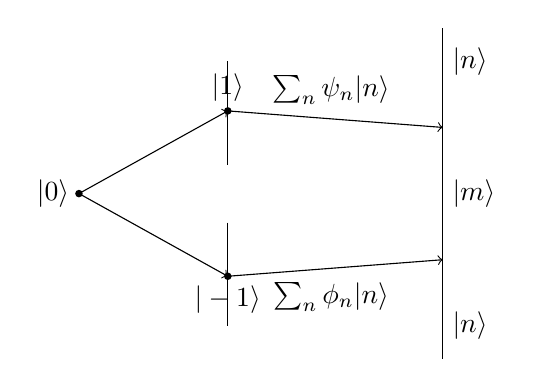
\begin{tikzpicture}[scale=1.05]
\fill (0,0) circle (1.3pt);
\node[left] at (0,0) {$|0\rangle$};

\draw (1.8,1.6) -- (1.8,0.35);
\draw (1.8,-0.35) -- (1.8,-1.6);
\fill (1.8,1) circle (1.3pt);
\fill (1.8,-1) circle (1.3pt);
\node[above] at (1.8,1) {$|1\rangle$};
\node[below] at (1.8,-1) {$|-1\rangle$};

\draw (4.4,2.0) -- (4.4,-2.0);
\node[right] at (4.4,1.6) {$|n\rangle$};
\node[right] at (4.4,0.0) {$|m\rangle$};
\node[right] at (4.4,-1.6) {$|n\rangle$};

\draw[->] (0,0) -- (1.8,1);
\draw[->] (0,0) -- (1.8,-1);
\draw[->] (1.8,1) -- (4.4,0.8);
\draw[->] (1.8,-1) -- (4.4,-0.8);

\node at (3.05,1.25) {$\sum_n \psi_n |n\rangle$};
\node at (3.05,-1.25) {$\sum_n \phi_n |n\rangle$};
\end{tikzpicture}
\caption{Версия двухщелевого эксперимента с конечным числом состояний: состояние источника \(|0\rangle\), два состояния щелей \(|1\rangle\) и \(|-1\rangle\) и базис экрана \(|n\rangle\).}
\end{figure}

\begin{figure}[htbp]
\centering
\includegraphics[width=0.68\textwidth]{lecture_06_figure_10.png}
\caption{Конечная решётка положений рядом с правилом линейной эволюции \(A\to A'\), \(B\to B'\).}
\lectureframe{01:18:00}
\end{figure}

По симметрии состояние источника эволюционирует в суперпозицию двух состояний щелей с равными амплитудами:
\begin{equation}
|0\rangle \longrightarrow |1\rangle+|-1\rangle.
\end{equation}
Теперь пусть состояние верхней щели эволюционирует в
\begin{equation}
|1\rangle \longrightarrow \sum_n \psi_n |n\rangle,
\end{equation}
а состояние нижней щели — в
\begin{equation}
|-1\rangle \longrightarrow \sum_n \phi_n |n\rangle.
\end{equation}
Стрелки здесь означают эволюцию во времени, а не равенство состояний в один и тот же момент. По линейности,
\begin{equation}
|1\rangle+|-1\rangle \longrightarrow \sum_n (\psi_n+\phi_n)|n\rangle.
\end{equation}
Это и есть ключевое правило. Амплитуды складываются до того, как образуются вероятности.

\begin{classroomqa}
\lecturetimestamp{01:21:59}
\audiencequestion{Как состояние щели \(|1\rangle\) может перейти в состояния, тоже помеченные целыми числами \(n\)? Означают ли эти кеты одно и то же место и время?}
\lecturerresponse{Метки относятся к разным моментам времени. \(|1\rangle\) обозначает электрон у верхней щели, тогда как \(|n\rangle\) справа обозначают возможные более поздние положения на экране. Стрелка — это эволюция во времени, а не равенство между одновременными конфигурациями.}
\end{classroomqa}

\begin{classroomqa}
\lecturetimestamp{01:25:30}
\audiencequestion{Должны ли амплитуды быть нормированы, и имеют ли они физическую размерность?}
\lecturerresponse{Полная эволюция должна сохранять полную вероятность; это и есть унитарность. Здесь общая нормировка опущена, потому что имеют значение только сложение и взаимное уничтожение амплитуд путей. Любые масштабные множители можно восстановить, когда состояние будет нормировано.}
\end{classroomqa}

Вероятность попадания в точку экрана \(m\) поэтому равна
\begin{align}
P_m &= |\psi_m+\phi_m|^2 \\
    &= |\psi_m|^2 + |\phi_m|^2 + \psi_m^*\phi_m + \phi_m^*\psi_m.
\end{align}
Первые 2 члена — это то, что дала бы классическая логика. Последние 2 — интерференционные члены.

\begin{figure}[htbp]
\centering
\includegraphics[width=0.68\textwidth]{lecture_06_figure_11.png}
\caption{Амплитуда для точки экрана и её четырёхчленное разложение вероятности на доске.}
\lectureframe{01:29:20}
\end{figure}

В симметричной точке экрана, обозначим её \(m=0\), симметрия подсказывает \(\psi_0=\phi_0\). Тогда
\begin{equation}
P_0 = |\psi_0+\phi_0|^2 = |2\psi_0|^2 = 4|\psi_0|^2.
\end{equation}
При открытых обеих щелях вероятность в этой точке оказывается в 4 раза больше, чем при одной открытой щели, а не в 2 раза. Это конструктивная интерференция.

Теперь введём фазовый сдвиг так, что \(\phi_0=-\psi_0\). Тогда
\begin{equation}
P_0 = |\psi_0-\psi_0|^2 = 0.
\end{equation}
Каждая щель сама по себе допускает попадание в эту точку, но если открыть обе сразу, попадание туда может стать невозможным. Это деструктивная интерференция. Сасскинд специально останавливается на том, насколько это странно: по его мнению, это столь же странно, как и Белл.

\begin{classroomqa}
\lecturetimestamp{01:33:14}
\audiencequestion{Что если фазовращатель или выбор щели изменяется только после того, как электрон уже летит? Нужно ли другой щели время, чтобы узнать об этом?}
\lecturerresponse{Ответ зависит от точной пространственно-временной конфигурации и от того, встречает ли электрон изменённую часть прибора. Квантовая механика эволюционирует состояние через реальную установку; вероятности по-прежнему получаются сложением применимых амплитуд. Предложение с отложенным выбором должно быть сформулировано строго, прежде чем можно будет оценивать утверждения о локальности.}
\end{classroomqa}

Теперь введём прибор. Есть одна дополнительная двухуровневая система — спин, первоначально находящийся в состоянии \(|d\rangle\). Если электрон проходит через верхнюю щель, он переворачивает этот спин в \(|u\rangle\). Если он проходит через нижнюю щель, то оставляет его неизменным. Начальное составное состояние есть \(|0,d\rangle\), и первое правило перехода принимает вид
\begin{equation}
|0,d\rangle \longrightarrow |1,u\rangle + |-1,d\rangle.
\end{equation}
Эта одна строка и есть весь смысл измерения в данной лекции. Положение электрона оказалось запутанным с записью, хранящейся в приборе.

\begin{figure}[htbp]
\centering
\includegraphics[width=0.66\textwidth]{lecture_06_figure_12.png}
\caption{Записи спина детектора вверх и вниз коррелированы с двумя альтернативами прохождения через щели.}
\lectureframe{01:44:10}
\end{figure}

\begin{classroomqa}
\lecturetimestamp{01:40:20}
\audiencequestion{Должен ли детектор стоять у обеих щелей?}
\lecturerresponse{Достаточно одного надёжного детектора. Если он регистрирует прохождение через верхнюю щель, то неизменившаяся запись указывает на нижнюю альтернативу, при условии что каждый прошедший электрон должен пройти через одно из двух отверстий. Второй детектор возможен, но лишь добавляет ещё одну подсистему, не меняя принципа.}
\end{classroomqa}

\begin{classroomqa}
\lecturetimestamp{01:40:51}
\audiencequestion{Почему бы не сказать, что электрон проходит через обе щели?}
\lecturerresponse{Без записи пути состояние является когерентной суперпозицией, и никакого ретроспективного факта о пути нет. При полном измерении, определяющем путь, прибор в каждом запуске регистрирует либо одну, либо другую альтернативу. Общей для обеих альтернатив является амплитуда состояния, а не две отдельно наблюдаемые траектории электрона.}
\end{classroomqa}

\begin{figure}[htbp]
\centering
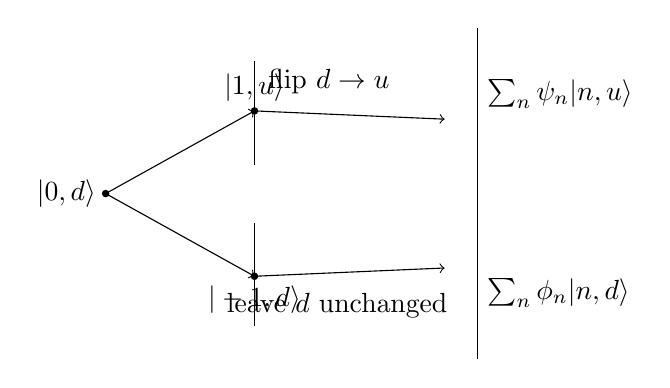
\begin{tikzpicture}[scale=1.05]
\fill (0,0) circle (1.3pt);
\node[left] at (0,0) {$|0,d\rangle$};

\draw (1.8,1.6) -- (1.8,0.35);
\draw (1.8,-0.35) -- (1.8,-1.6);
\fill (1.8,1) circle (1.3pt);
\fill (1.8,-1) circle (1.3pt);
\node[above] at (1.8,1) {$|1,u\rangle$};
\node[below] at (1.8,-1) {$|-1,d\rangle$};

\draw (4.5,2.0) -- (4.5,-2.0);
\node[right] at (4.5,1.2) {$\sum_n \psi_n |n,u\rangle$};
\node[right] at (4.5,-1.2) {$\sum_n \phi_n |n,d\rangle$};

\draw[->] (0,0) -- (1.8,1);
\draw[->] (0,0) -- (1.8,-1);
\draw[->] (1.8,1) -- (4.1,0.9);
\draw[->] (1.8,-1) -- (4.1,-0.9);

\node at (2.7,1.35) {flip \(d\to u\)};
\node at (2.8,-1.35) {leave \(d\) unchanged};
\end{tikzpicture}
\caption{Измерение как запутывание со спином детектора. Верхний путь переворачивает спин прибора; нижний путь оставляет его без изменения.}
\end{figure}

Предположим, как и в лекции, что по пути к экрану со спином больше ничего не происходит. Тогда
\begin{align}
|1,u\rangle &\longrightarrow \sum_n \psi_n |n,u\rangle, \\
|-1,d\rangle &\longrightarrow \sum_n \phi_n |n,d\rangle.
\end{align}
Следовательно, конечное состояние при открытых обеих щелях имеет вид
\begin{equation}
|\Psi_{\mathrm{final}}\rangle
  = \sum_n \psi_n |n,u\rangle + \sum_n \phi_n |n,d\rangle.
\end{equation}
Это не суперпозиция состояний одного только электрона. Это запутанное состояние электрона и прибора.

\begin{figure}[htbp]
\centering
\includegraphics[width=0.68\textwidth]{lecture_06_figure_13.png}
\caption{Амплитуды для двух путей достигают экрана, неся ортогональные записи прибора.}
\lectureframe{01:47:35}
\end{figure}

Самый прямой способ вычислить вероятность попадания в точку \(m\) — использовать проектор на эту точку в электронной подсистеме:
\begin{equation}
\Pi_m = |m\rangle\langle m|\otimes I_{\mathrm{spin}}.
\end{equation}
Применяя \(\Pi_m\) к конечному состоянию, получаем
\begin{equation}
\Pi_m |\Psi_{\mathrm{final}}\rangle
= |m\rangle\bigl(\psi_m|u\rangle+\phi_m|d\rangle\bigr).
\end{equation}
Следовательно, вероятность прихода в \(m\) равна
\begin{align}
P_m
  &= \langle \Psi_{\mathrm{final}}|\Pi_m|\Psi_{\mathrm{final}}\rangle \\
  &= \bigl(\psi_m^*\langle u|+\phi_m^*\langle d|\bigr)
     \bigl(\psi_m|u\rangle+\phi_m|d\rangle\bigr) \\
  &= |\psi_m|^2 + |\phi_m|^2
     + \psi_m^*\phi_m\langle u|d\rangle
     + \phi_m^*\psi_m\langle d|u\rangle.
\end{align}
Но состояния записи ортогональны:
\begin{equation}
\langle u|d\rangle=0.
\end{equation}
Поэтому перекрёстные члены исчезают:
\begin{equation}
P_m = |\psi_m|^2 + |\phi_m|^2.
\end{equation}
Это и есть главный математический вывод лекции. Как только информация о пути записана, интерференция исчезает, и вероятности складываются классическим образом.

\begin{classroomqa}
\lecturetimestamp{01:49:09}
\audiencequestion{В чём различие между суперпозицией \(|1\rangle+|-1\rangle\) и состоянием \(|1,u\rangle+|-1,d\rangle\)?}
\lecturerresponse{В первом случае речь идёт об одной системе в линейной комбинации двух положений; нет ничего другого, с чем она могла бы быть запутана. Во втором случае речь идёт о двух системах, и путь коррелирован со спином детектора. Тогда считывание спина раскрывает информацию о пути.}
\end{classroomqa}

\section{Записи окружения и частичное измерение}

Специально сконструированный детектор — не единственный регистратор. Атом возле щели, остаточный газ, нагретая поверхность или любая другая степень свободы могут скоррелироваться с путём. Если её конечные состояния — \(|E_1\rangle\) и \(|E_2\rangle\), то состояние имеет вид
\begin{equation}
|\Psi\rangle
=\sum_n\left(\psi_n|n\rangle|E_1\rangle
+\phi_n|n\rangle|E_2\rangle\right).
\end{equation}
Интерференционные члены теперь умножаются на перекрытие \(\langle E_1|E_2\rangle\). Ортогональные записи делают пути полностью различимыми и полностью устраняют интерференцию. Совпадающие записи оставляют \(\langle E_1|E_2\rangle=1\) и сохраняют интерференцию. Промежуточное перекрытие даёт частичную видимость интерференции.

\begin{figure}[htbp]
\centering
\includegraphics[width=0.68\textwidth]{lecture_06_figure_14.png}
\caption{Перекрывающиеся и разделённые волновые пакеты окружения иллюстрируют частичную и полную запись о пути.}
\lectureframe{01:53:40}
\end{figure}

\begin{classroomqa}
\lecturetimestamp{01:50:48}
\audiencequestion{Запутается ли обычный атом возле щели с пролетающим электроном, даже если никто специально за ним не наблюдает?}
\lecturerresponse{Да. Здесь существенно не знание, а физическая корреляция. Если атом или окружающий газ возмущён настолько, что его последующее состояние различает пути, то тем самым записывается информация о том, по какому пути прошёл электрон, и подавляется интерференция. Поэтому такие эксперименты требуют изоляции, низких температур и часто слабо взаимодействующих частиц, таких как фотоны.}
\end{classroomqa}

Охлаждение приводит степени свободы окружения в состояния, близкие к основным, и уменьшает случайные записи. Энергетическая щель тоже помогает: если налетающая частица не может передать минимальную энергию возбуждения, окружение может оказаться неспособным сохранить информацию о пути. Напротив, заряженные частицы могут возмущать соседнее вещество своими электрическими полями, что делает интерференцию электронов особенно трудной для реализации.

\begin{classroomqa}
\lecturetimestamp{01:54:49}
\audiencequestion{Можно ли действительно получить интерференционную картину с одиночными электронами?}
\lecturerresponse{Каждый электрон оставляет только одно локализованное попадание. Пропускайте частицы по одной, с достаточным разнесением, чтобы они не могли взаимодействовать, и накапливайте много повторений. Накопленное частотное распределение показывает интерференционную картину; одно событие само по себе — лишь отдельная точка.}
\end{classroomqa}

\begin{classroomqa}
\lecturetimestamp{01:55:59}
\audiencequestion{Разрушает ли измерение запутанность или создаёт её?}
\lecturerresponse{Взаимодействие, определяющее путь, создаёт запутанность между системой и прибором, и именно эта запутанность уничтожает интерференцию между альтернативами. Более позднее измерение может скоррелировать прибор ещё с одной системой и может обусловить оставшееся состояние, поэтому всегда нужно уточнять, о каких двух подсистемах и о какой интерференции идёт речь.}
\end{classroomqa}

\begin{classroomqa}
\lecturetimestamp{01:57:44}
\audiencequestion{Можно ли ослабить взаимодействие так, чтобы прибор получал лишь частичную информацию о пути?}
\lecturerresponse{Да. Слабое взаимодействие может переворачивать спин детектора лишь с некоторой амплитудой, оставляя неортогональные состояния записи. Тогда пути различимы лишь частично, и интерференция ослабляется лишь частично. Более сильное измерение означает большую различимость, более сильную запутанность с записью и меньшую видимость интерференционных полос.}
\end{classroomqa}

Поэтому релевантный здесь коллапс вполне конкретен: это исчезновение перекрёстных членов, когда информация о пути записана в другой системе. При отсутствии записи амплитуды складываются. При полностью различимых записях их скалярные произведения обращаются в нуль, и складываются вероятности. Между этими крайностями сила измерения и видимость интерференции меняются непрерывно.
